%\documentclass[11pt]{article}
%\usepackage{fullpage}

%\begin{document}

\subsection{Implementation Choices}
\textbf{Database Implementation}\\

The Database layer will be composed by two different datbases: a relational database and a NoSQL database. The implementation choices for the realtional one are the following:
\begin{itemize}
\item MySQL 5.7 as the relational DBMS
\item InnoDB as the subsiding database engine; InnoDB is a good choice for this application, because it manages concurrent access to the same tables in a very clean and quick way
\item The Java Persistence API (JPA) within the Application Server will serve as an interface with the Database
\end{itemize}

The NoSQL Database is in charge of storing all the data generated by the system such as logs and all the kinds of data that  will not require any update or delete during the time and that will be accessed to consulted only. The decision of using a NoSQL database instead of a traditional relational database is driven by the need of speed in inserting and accessing a big amount of data.For this reason, it's not required to ensure all the ACID properties over transaction. The NoSQL Database runs on MongoDB as DBMS and communicates logic tier using TCP/IPO protocol on an arbitrary port.

Both databases must be physically protected and duplicated in order to avoid loss. Communication must be encrypted and different users should be created and assigned to the different softwares that access the database in order to always guarantee the minimum required level of privileges per software.\\

\hspace{-\parindent}\textbf{Application Server Implementation}\\

The main choice for this layer is the use of Java Enterprise Edition 7 (JEE). This was the most reasonable option for several reasons: the final product is a large-scope application, and thus needs distribution to great numbers of clients simultaneously; for the same reason, it needs to satisfy continuously evolving functional requirements and customer demands; JEE also allows the developers to focus on the logic behind the main functionalities while being supported by a series of reliable APIs and tools that, among other features, can guarantee the main non-functional requirements of the case (e.g. security, reliability, availability...); lastly, it can reduce the complexity of the application by using mechanisms and models that easily adapt to a large-scale project. 

The specific implementation choices are:
\begin{itemize}
\item GlassFish Server as the Application Server implementation
\item Enterprise JavaBeans (EJB) to implement the single business logic modules described in the sections above using Stateless Beans. These will be appropriately subdivided into EJB containers as specified by the JEE documentation
\item Java Persistence API (JPA) as persistence unit to perform the Database access, that is not implemented with direct SQL queries. Entity beans will be used to implement the object representation of the database entities and they are strictly related to the entities of the E-R diagram (Figure 3). The detailed relationships between the individual session beans and the various entity beans will be described in Section \textbf{XXX}
\item JAX-RS to implement proper RESTful APIs to interface with clients
\item To interface with external systems, existing RESTful APIs defined by the partners will be used in the communication with the payment handlers, whereas a dedicated one will be provided to the maintenance system to interact properly with the application services
\end{itemize}
\begin{center}
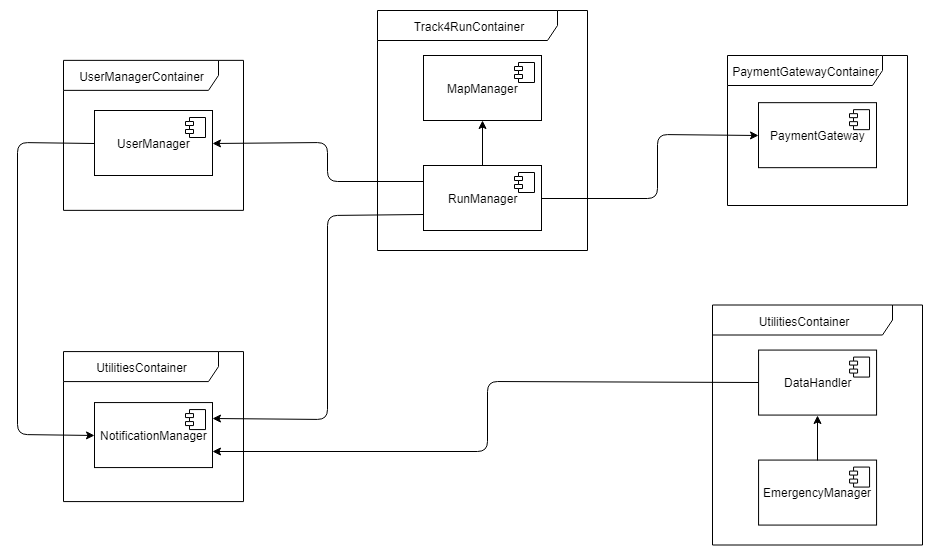
\includegraphics[scale=0.5]{sections/diagrams/component_view.png}
\newline
\captionof{figure}{The components of the Application Server	implemented as session	beans to develop the business logic.	The detailed interface of each bean	is thoroughly described	in section \textbf{XXX}. An arrow going from component C1 to component C2 means that C1 uses interfacing methods provided	by C2.}
\end{center}

\hspace{-\parindent}\textbf{Mobile Application Client Implementation}\\

The mobile application UI must be designed following the design guidelines provided by the devices’ manufacturers. Two architectures must be supported: iOS and Android. The iOS application must be written in Swift, while the Android one must be implemented in Java.

The core of both application must be a Controller that communicates user inputs (after translating them from the UI input) to the Application Server via RESTful APIs. The access to the GPS of the devices and HealthData of users (only for devices that can collect these kind of data) must be performed through the default frameworks of the respective systems.
\begin{center}
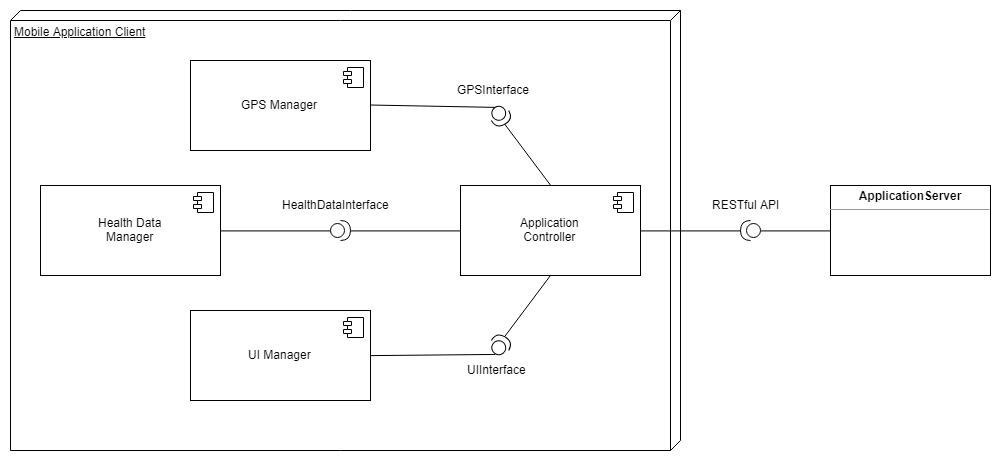
\includegraphics[scale=0.45]{sections/diagrams/mac.png}
\newline
\captionof{figure}{The components of the mobile application}
\end{center}

\clearpage
%\end{document}